\documentclass[11pt,a4paper]{article}

\usepackage[utf8]{inputenc}
\usepackage[T1]{fontenc}
\usepackage{lmodern}
\usepackage{microtype}
\usepackage[margin=1in]{geometry}
\usepackage{graphicx}
\usepackage{amsmath,amssymb}
\usepackage{booktabs}
\usepackage{multirow}
\usepackage{array}
\usepackage{caption}
\captionsetup{font=small,labelfont=bf,labelsep=period}
\usepackage{subcaption}
\usepackage{hyperref}
\hypersetup{colorlinks=true,linkcolor=blue!60!black,citecolor=blue!50!black,urlcolor=blue!60!black}
\usepackage[numbers,sort&compress]{natbib}
\usepackage{authblk}
\usepackage{xcolor}
\usepackage{tcolorbox}

\title{\textbf{Phase-Localised Pose Correlates of Driver Distance in a Small-$N$ Golf Corpus:\\[2pt]
A Secondary, Associative Analysis of CaddieSet}}

\author[1]{Edward Xiong}
\affil[1]{Independent Research}
\date{}

\begin{document}
\maketitle

\begin{abstract}
\noindent
The \emph{CaddieSet} corpus~\citep{jung2025caddieset} contains 1{,}757 swings from \textbf{only $N=8$ golfers}
paired with launch-monitor outcomes, enabling a secondary analysis of which body-posture features at which swing
phases are associated with driver distance, ball speed, and directional accuracy.  We ask: given this small-$N$,
within-subject structure, how much signal survives (i) extreme-groups inflation of Cohen's $d$, (ii)
Benjamini--Hochberg multiple-testing control across 252 feature $\times$ phase $\times$ outcome tests, and
(iii) golfer-aware cross-validation?  Four findings emerge.  First, 98 of 252 pose--outcome associations survive
BH-FDR $q<0.05$, concentrated in mid-backswing lead-arm angle and early/pre-impact hip lateral shift; the
continuous-Pearson back-transform of the largest extreme-groups $d=1.36$ is $r\approx0.39$.  Second, random
5-fold CV $R^2$ for pose-only Random Forests is $0.50$ for driver distance, but GroupKFold(8) CV grouped by
golfer collapses the same ceiling to $R^2=-4.36$: the headline prediction number on CaddieSet is dominated by
memorising golfer identity.  Third, $K$-means in the pose space produces clusters with silhouette $=0.54$ and
mean leave-one-golfer-out Adjusted Rand Index $=0.956$, but the four-cluster solution assigns $83$--$89\%$ of
two of the clusters to single golfers, so the clusters should be read as mixed swing + identity factors rather
than pure biomechanical archetypes.  Fourth, a depth-3 regression tree surrogate reaches random CV $R^2=0.34$
but $-3.36$ under GroupKFold; its seven leaves carry wide bootstrap CIs and describe the \emph{within-sample}
structure of distance in these eight golfers only.  We conclude that CaddieSet --- with its current golfer
count --- supports within-subject, descriptive biomechanical claims, but does not support population-level
prescriptive rules.  We release code and an extended artefact set so that follow-up corpora can retest every
claim in minutes.\footnote{Code, artefacts and figures:
\url{https://github.com/edwardxiong2027/caddieset-rules}.}
\end{abstract}

\vspace{0.8em}
\begin{center}
\begin{tcolorbox}[colback=gray!5,colframe=gray!40,width=0.96\linewidth]
\small
\textbf{Keywords:} golf biomechanics, human pose estimation, interpretable machine learning, golfer-aware
cross-validation, multiple-testing correction, subject variability, CaddieSet.
\end{tcolorbox}
\end{center}

\section{Introduction}

Golf has long been an attractive test-bed for data-driven biomechanics: a small number of postural decisions, made
in roughly 1.2--1.5\,s of body motion, determine an outcome that rolls out over hundreds of yards.  Classical
studies using marker-based motion capture established the canonical view of the swing as a kinetic chain in which
a delayed pelvis--thorax separation (the ``X-factor'') is built during the backswing and released through the
downswing \citep{cheetham2001xfactor,nesbit2005sixdof,meister2011rotational}.  Quantitative reviews
\citep{hume2005biomechanics} conclude that both \emph{distance} and \emph{accuracy} arise from the same kinetic
chain, but through different mechanisms: distance is dominated by clubhead speed (driven by upper--lower body
separation), whereas accuracy depends more on impact-phase club geometry.

The recent CaddieSet dataset~\citep{jung2025caddieset} broadens access by pairing phase-segmented joint features
with launch-monitor ball metrics --- at the cost of sampling only \textbf{eight golfers}.  Our first goal in this
paper is to revisit the CaddieSet corpus with a small-$N$, secondary-analysis lens, and to measure how much
biomechanical signal remains after we (a) correct extreme-groups effect-size inflation, (b) apply
Benjamini--Hochberg FDR control across the full feature grid, and (c) evaluate predictive claims under
\emph{golfer-aware} cross-validation grouped by subject identity.

Our guiding questions are:
\begin{description}
    \item[Q1 --- Effect-size map with FDR control.]
        For each (phase, view, outcome), which body-posture features remain significantly associated with
        ball flight after BH-FDR correction, and how large are the effects on the continuous (not extreme-groups)
        scale?
    \item[Q2 --- Predictive ceilings, honestly.]
        How do the pose-only predictive ceilings \emph{change} when we replace random KFold with GroupKFold(8)
        grouped by golfer?
    \item[Q3 --- Archetype discovery or identity leakage?]
        Do pose-space clusters reflect biomechanical \emph{styles}, or do they primarily track golfer identity?
    \item[Q4 --- Rule surrogates, transparently.]
        Can a shallow tree compress the strongest within-sample associations into a human-readable structure
        while reporting both within- and between-golfer generalisation?
\end{description}

Figure~\ref{fig:pipeline} summarises the pipeline.  Our contributions are:
\begin{enumerate}
    \item A phase-$\times$-outcome effect-size map with FDR-significance masking (Fig.~\ref{fig:heatmap}) and
          a Fitzsimons/Cohen back-transform of the extreme-groups effect sizes to approximate continuous
          Pearson $r$.
    \item A direct measurement of the \emph{identity gap}: random 5-fold CV $R^2$ for distance is $0.50$ but
          collapses to $R^2=-4.36$ under GroupKFold(8) (Fig.~\ref{fig:ceiling}).
    \item A validated clustering pipeline that reports silhouette vs.\ a null-label baseline, per-golfer $\times$
          cluster crosstab, and leave-one-golfer-out Adjusted Rand Index --- documenting that two of the four
          clusters are golfer-dominated.
    \item A shallow regression-tree surrogate reported with depth-sweep sensitivity, leaf-level bootstrap CIs,
          and an honest GroupKFold $R^2$ of $-3.36$, together with a sensitivity grid showing the power/accuracy
          gap is robust to target transform and model family.
\end{enumerate}
We read the results as descriptive, not prescriptive: they describe what covaries with outcome \emph{within
these eight golfers}.

\begin{figure}[t]
\centering
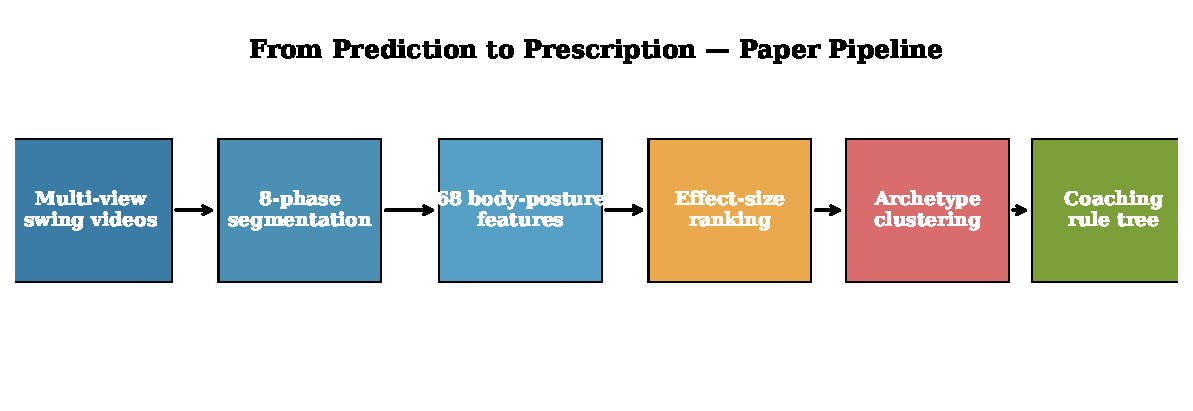
\includegraphics[width=0.98\linewidth]{figures/fig1_pipeline.pdf}
\caption{Secondary-analysis pipeline.  Inputs (blue) are inherited from \citet{jung2025caddieset}.
         Associative/descriptive stages (yellow/red/green) are contributed by this paper.  All inference
         uses golfer-aware cross-validation and BH-FDR correction.}
\label{fig:pipeline}
\end{figure}

\section{Related Work}
\label{sec:related}

\paragraph{Golf biomechanics and performance.}
\citet{chu2010kinematic} report that 4--6 biomechanical variables explain $\sim$56\% of driving performance
variance in low-handicap golfers --- a reference point for our ceiling analysis.
\citet{langdown2012footpressure} links stance width to ground-reaction-force patterns that gate distance.
\citet{macdougall2021putting} isolate kinematic predictors of clubhead speed in elite golfers.  These studies
typically use dozens of subjects recorded under controlled conditions; we operate on a considerably smaller
golfer pool (8) with single-camera pose features, which shapes the claims we can responsibly make.

\paragraph{Pose estimation for sport.}
General-purpose human-pose models \citep{cao2019openpose,sun2019hrnet,xu2022vitpose} have made it practical to
extract joint-level features from single-camera sports video.  The GolfDB benchmark~\citep{mcnally2019golfdb}
introduced swing-sequencing as a fine-grained video task, and \citet{liao2022maniflow} extended the
phase-segmentation problem; the \citet{ke2023golfpose} survey situates these within the broader pose-for-golf
literature.  CaddieSet~\citep{jung2025caddieset} is (to our knowledge) the first public corpus pairing
phase-segmented joint features with launch-monitor ball data.

\paragraph{Interpretable rule extraction.}
A large body of work targets rule-based surrogates for tabular prediction: Bayesian Rule Lists
\citep{letham2015rules}, Interpretable Decision Sets \citep{lakkaraju2016interpretable}, certifiably optimal
rule lists (\textsc{CORELS}) \citep{angelino2017corels}, rule ensembles \citep{friedman2008rulefit}, and
super-sparse linear integer models \citep{ustun2016slim}.  We use the simplest member of this family --- a
depth-3 regression tree --- so that the surrogate is directly inspectable; we do not claim our tree is the
best-in-class rule representation for this problem.  \citet{rudin2019stop} and
\citet{doshivelez2017interpretability} motivate the broader preference for interpretable models in
high-stakes or coaching-adjacent settings.

\paragraph{Multiple testing and subject variability.}
\citet{benjamini1995controlling} introduced the Benjamini--Hochberg procedure that we use to control FDR across
252 feature--outcome tests.  \citet{fitzsimons2008correction} and \citet{cohen1983dichotomization} quantify the
systematic inflation introduced by extreme-groups / dichotomised comparisons relative to continuous effect
sizes --- the reason we back-transform point-biserial $r$ to an approximate continuous $r$.
\citet{bartlett2006subject} and \citet{button2003coordination} document that inter-individual variability in
sport movement is large enough to dominate pooled-group analyses, motivating our GroupKFold(8) evaluation and
our per-golfer cluster crosstabs.

\paragraph{Positioning.}
The closest prior work is the CaddieSet paper itself \citep{jung2025caddieset}, which benchmarks predictors
trained on 15 expert-defined summary metrics.  We are complementary but differ in three ways: we use \emph{all
68} per-phase pose features directly rather than curated summaries; we rank by effect size with explicit FDR
control; and we report every downstream model under both random and golfer-aware cross-validation so that the
identity gap is visible rather than hidden.

\section{Dataset and Features}
\label{sec:data}

We use CaddieSet~\citep{jung2025caddieset} without modification.  The corpus contains $N=1{,}757$ swings from
\textbf{8 golfers}, split across two camera views (Face-On $n=924$, Down-the-Line $n=833$) and 8 clubs, with the
driver (W1) dominating ($n=1{,}137$, 65\%).  Each swing is labelled with five ball-flight outcomes (Distance,
Carry, DirectionAngle, SpinBack, SpinSide, BallSpeed) and 68 body-posture features indexed by a phase prefix
$\{0,\dots,7\}$ corresponding to Address, Takeaway, Mid-backswing, Top-of-backswing, Early-downswing,
Pre-impact, Impact, and Finish.  Roughly half of the features are populated only in one camera view; we
therefore run all analyses \emph{per-view} to avoid imputation bias.  Summary statistics by club
(means $\pm$ within-club SD) are in Table~\ref{tab:clubs}.

\begin{table}[t]
\centering
\small
\caption{Ball-flight summaries per club (mean $\pm$ SD).  SDs include within- and between-golfer variation.}
\label{tab:clubs}
\begin{tabular}{lrrrr}
\toprule
\textbf{Club} & \textbf{Distance (yd)} & \textbf{Carry (yd)} & \textbf{Ball Speed (m/s)} & \textbf{Back Spin (rpm)} \\
\midrule
W1 (Driver)  & $189.5 \pm 29.9$ & $171.1 \pm 28.1$ & $56.3 \pm 6.0$ & $2{,}269 \pm 618$ \\
W3 (3-Wood)  & $196.6 \pm 18.6$ & $177.6 \pm 17.2$ & $58.2 \pm 3.6$ & $2{,}508 \pm 564$ \\
I4           & $167.3 \pm 16.2$ & $151.5 \pm 15.1$ & $51.5 \pm 3.2$ & $3{,}242 \pm 715$ \\
I5           & $160.1 \pm 14.1$ & $144.1 \pm 12.8$ & $49.6 \pm 2.9$ & $3{,}123 \pm 678$ \\
I6           & $149.8 \pm 13.9$ & $137.0 \pm 12.4$ & $48.7 \pm 2.7$ & $4{,}103 \pm 752$ \\
I7           & $137.2 \pm 13.4$ & $125.7 \pm 12.5$ & $45.8 \pm 2.8$ & $4{,}562 \pm 717$ \\
I8           & $133.4 \pm 12.8$ & $123.5 \pm 11.9$ & $45.6 \pm 2.6$ & $5{,}303 \pm 707$ \\
I9           & $128.2 \pm 12.1$ & $118.0 \pm 11.4$ & $44.3 \pm 2.4$ & $5{,}133 \pm 692$ \\
\bottomrule
\end{tabular}
\end{table}

\paragraph{Note on feature semantics.}
The public release exposes descriptive English-prefixed column names (\texttt{LEFT-ARM-ANGLE},
\texttt{HIP-SHIFTED}, \texttt{HANGING-BACK}, \dots) but does not publish a formal data dictionary of units or
sign conventions.  We interpret signs following the most natural biomechanical reading (e.g.\ a larger
\texttt{LEFT-ARM-ANGLE} corresponds to a straighter lead arm, a positive \texttt{HIP-SHIFTED} corresponds to the
pelvis being shifted target-ward of Address).  This is an \emph{assumed} interpretation; see
Section~\ref{sec:limits} for how this affects the strength of our claims.

\section{Methodology}
\label{sec:method}

All subsequent analyses focus on driver swings (W1) to keep club-type confounding out of the effect-size
calculation.

\subsection{Effect sizes with FDR control}
For each (view, outcome, feature), we compute three quantities:
\begin{itemize}
    \item \textbf{Extreme-groups Cohen's $d$} between the top- and bottom-20\% outcome groups.  This is the
          headline number in many coaching-style analyses and is \emph{systematically inflated} relative to the
          continuous effect \citep{cohen1983dichotomization}.
    \item \textbf{Point-biserial $r$} from the two-sample $t$-statistic, then the Fitzsimons back-transform
          \citep{fitzsimons2008correction} to an \emph{approximate continuous Pearson $r$}:
          $\;\;r_{\text{cont}} \approx r_{\text{pb}} \cdot \sqrt{p(1-p)} / \varphi(\Phi^{-1}(p))$,
          with $p=0.2$.
    \item \textbf{Full-sample Pearson $r$ and Spearman $\rho$} against the \emph{signed} outcome, so that the
          extreme-groups and continuous measures can be cross-checked.
\end{itemize}
We run all $252 = 63\,\text{features} \times 2\,\text{views} \times 2\,\text{targets}$ tests as a single grid
and apply the Benjamini--Hochberg FDR procedure \citep{benjamini1995controlling} to the Pearson $p$-values,
reporting $q$-values and the subset surviving $q<0.05$.  Absolute-valued targets are used for direction error
and side spin so that magnitude, not side, is ranked.

\subsection{Predictive ceilings: random KFold vs.\ GroupKFold(8)}
We fit Random-Forest regressors \citep{breiman2001randomforest} (300 trees, \texttt{min\_samples\_leaf}$=5$) on
all features with $>$90\% non-null density in a given view, after $[0.1\%,99.9\%]$ winsorisation and
median-imputation.  For each (view, target) we report \emph{both} random 5-fold $R^2$ (the number the original
CaddieSet benchmarks use) \emph{and} $\texttt{GroupKFold}(n_\text{splits}=8)$ $R^2$ grouped by golfer, where
no golfer's swings appear in both training and test folds.  The gap between the two is itself the answer to
whether pose-only generalisation is population-level or identity-level.

\subsection{Archetype validation}
On the Face-On $\times$ W1 subset ($n=613$), we winsorise at $[1\%,99\%]$, apply a \texttt{RobustScaler}, and
run $K$-means for $K\in\{2,\dots,10\}$.  For each $K$ we compute silhouette, Davies--Bouldin, and a \emph{null
silhouette baseline} obtained by randomly permuting cluster labels while preserving cluster sizes.  We then
fix $K=4$ and report (i) per-golfer $\times$ per-cluster contingency, (ii) entropy of each cluster over
golfers, and (iii) leave-one-golfer-out (LOGO) stability via the Adjusted Rand Index between the full-sample
clustering and a re-fit clustering that excludes one golfer.  UMAP \citep{mcinnes2018umap} is used only for
visualisation, not for clustering.

\subsection{Rule surrogate}
We fit a \texttt{DecisionTreeRegressor} (\texttt{max\_depth}=3, \texttt{min\_samples\_leaf}=30) on the same
subset, targeting Distance.  Two points differ from the original pipeline and are important:
\begin{itemize}
    \item \textbf{No feature-selection leak.}  The tree receives every Face-On feature and performs its own
          split selection inside each cross-validation fold.  No upstream importance ranking is used to prune
          the input set.
    \item \textbf{Depth sweep + per-leaf bootstrap CIs.}  Depths $d=2,\dots,5$ are evaluated under both random
          and GroupKFold CV; for the chosen depth-3 tree, each leaf's mean Distance is reported with a 2{,}000-resample
          percentile 95\% bootstrap CI, so small leaves' point estimates come with explicit uncertainty.
\end{itemize}

\subsection{Robustness of the accuracy ceiling}
\label{sec:method-robust}
To test whether the power-vs-accuracy gap is an artefact of the $|\cdot|$ transform or the Random Forest choice,
we rerun the ceiling analysis with three target variants --- signed, $|y|$, and $\sqrt{|y|}$ --- for both
DirectionAngle and SpinSide, and with two model families: Random Forest (as above) and
\texttt{HistGradientBoostingRegressor}.  All six target variants are reported under both random and
GroupKFold(8).

\subsection{Implementation}
All analyses use Python 3.10, \texttt{scikit-learn} \citep{pedregosa2011scikit}, \texttt{umap-learn}, and
\texttt{matplotlib}.  Seeds are fixed (42) throughout.  A single \texttt{make} invocation reproduces every
artefact, table, and figure in this paper.

\section{Results}

\subsection{Phase-$\times$-outcome effect-size map with FDR control}
\label{sec:phase-map}

Across the 252-cell test grid, \textbf{98 cells survive BH-FDR at $q<0.05$} (39\% of the grid).
Figure~\ref{fig:heatmap} plots the maximum $|d|$ in each (view, target, phase) tile and hatches the tiles in
which \emph{no} feature survives FDR correction.  Three regularities are robust after FDR control:

\begin{enumerate}
    \item \textbf{Power signals are concentrated late in the backswing and early in the downswing.}
          In Face-On the largest FDR-surviving effects for Distance and Ball Speed occur at phase 2
          (Mid-backswing lead-arm angle, $d=1.19$, continuous-$r$ back-transform $\approx 0.39$) and phase 4
          (Early-downswing hip shift, $d=1.36$, $r_{\text{cont}}\approx 0.45$).  In Down-the-Line the peak
          shifts to phase 3 (Top of backswing, right-leg angle, $d=-1.40$, $r_{\text{cont}}\approx -0.46$).
    \item \textbf{Accuracy signals are weaker and more dispersed.}
          Max $|d|$ for direction error never exceeds $0.81$, and many accuracy cells do not survive FDR.
          The continuous $r_{\text{cont}}$ for the strongest accuracy feature is only $\approx 0.27$.
    \item \textbf{Views are complementary, not redundant.}
          Face-On localises the strongest distance signals at phases 4--5; DTL localises them at phases 0--3.
          A deployment using one view leaves measurable signal on the table in the other.
\end{enumerate}

\begin{figure}[t]
\centering
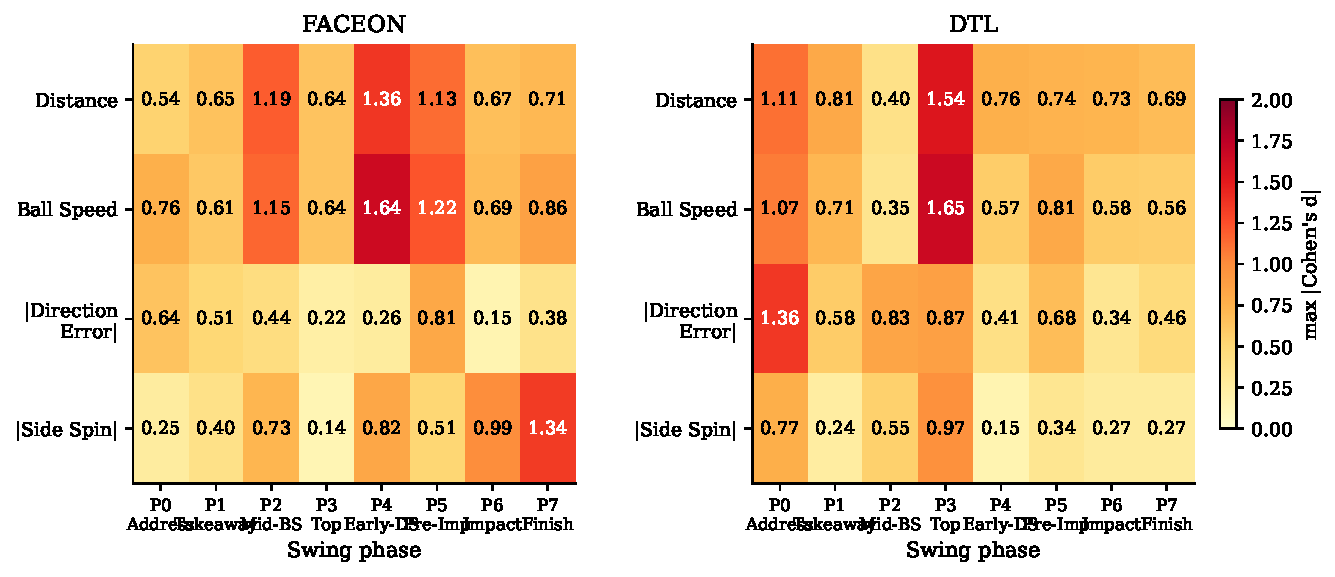
\includegraphics[width=0.99\linewidth]{figures/fig2_heatmap.pdf}
\caption{Phase $\times$ outcome effect-size map for driver swings; each cell is the maximum extreme-groups
         $|d|$ in that tile.  Cells in which no feature survives BH-FDR $q<0.05$ are hatched and marked with an
         asterisk.  The headline extreme-groups effects ($d>1$) back-transform to continuous Pearson $r$ in
         the $0.39$--$0.46$ range, consistent with moderate --- not near-deterministic --- associations.}
\label{fig:heatmap}
\end{figure}

\subsection{The power/accuracy gap --- and the identity gap}
\label{sec:ceiling}

Figure~\ref{fig:ceiling} compares random 5-fold CV $R^2$ (the number the field usually quotes) with
GroupKFold(8) grouped by golfer, for each (view, outcome).

\textbf{Random CV reproduces the apparent power/accuracy gap.}  Pose-only Random Forests reach $R^2\approx
0.48\text{--}0.56$ for distance and ball speed but only $0.12\text{--}0.34$ for directional accuracy and side
spin --- consistent with the biomechanical intuition that accuracy is gated by millimetre-scale impact geometry
that pose features only indirectly capture.

\textbf{GroupKFold replaces the story.}  With no single golfer's swings in both train and test, all four
outcomes collapse to negative $R^2$: for distance, $-4.36$ (Face-On) and $-3.72$ (DTL); for ball speed,
$-4.67$ and $-4.70$; for $|$direction error$|$, $-0.49$ and $-0.51$; for $|$side spin$|$, $-0.37$ and
$-0.32$.  A negative CV $R^2$ means the model predicts a held-out golfer \emph{worse} than simply predicting
the global mean.  The honest interpretation is that the $R^2 \approx 0.5$ distance ceiling on CaddieSet is
largely the model memorising golfer identity; pose alone, in this 8-golfer corpus, does not generalise across
subjects.  The accuracy outcomes are less affected by the switch because they had little to memorise to begin
with.

\begin{figure}[t]
\centering
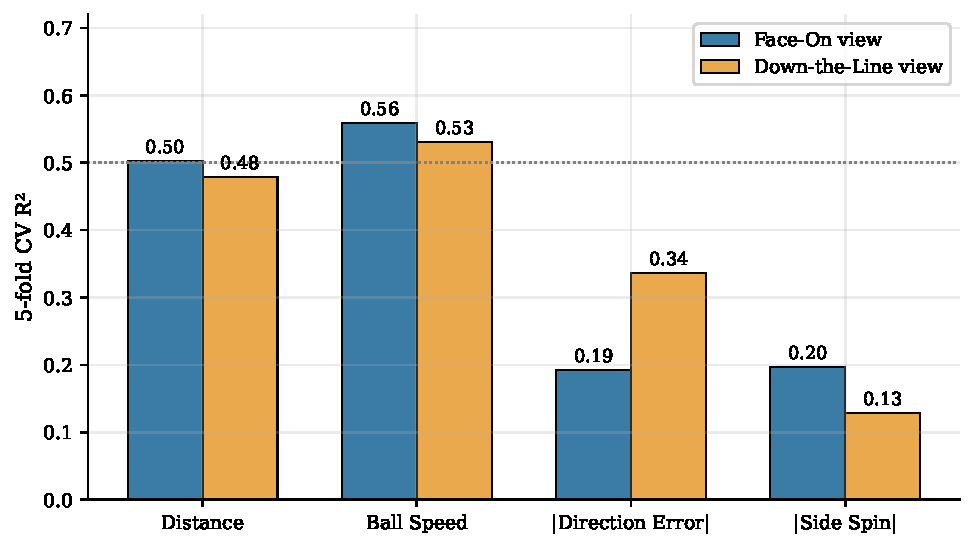
\includegraphics[width=0.98\linewidth]{figures/fig5_ceiling.pdf}
\caption{Predictive ceiling of pose-only Random Forests per (view, outcome) under random 5-fold (blue) and
         GroupKFold(8) grouped by golfer (red).  The gap between the two bars is the identity gap: how much
         of the random-CV ceiling reflects memorising which golfer hit the shot.}
\label{fig:ceiling}
\end{figure}

Figure~\ref{fig:robustness} shows this is not an artefact of the $|\cdot|$ transform nor of Random Forests.
For both DirectionAngle and SpinSide, across signed / $|y|$ / $\sqrt{|y|}$ transforms and across Random Forest
vs.\ HistGradientBoosting, random-CV $R^2$ is positive and GroupKFold $R^2$ is negative.  Signed direction
actually gives the highest random $R^2$ of the six variants (0.385 Face-On RF), but still collapses under
GroupKFold ($-0.31$).

\begin{figure}[t]
\centering
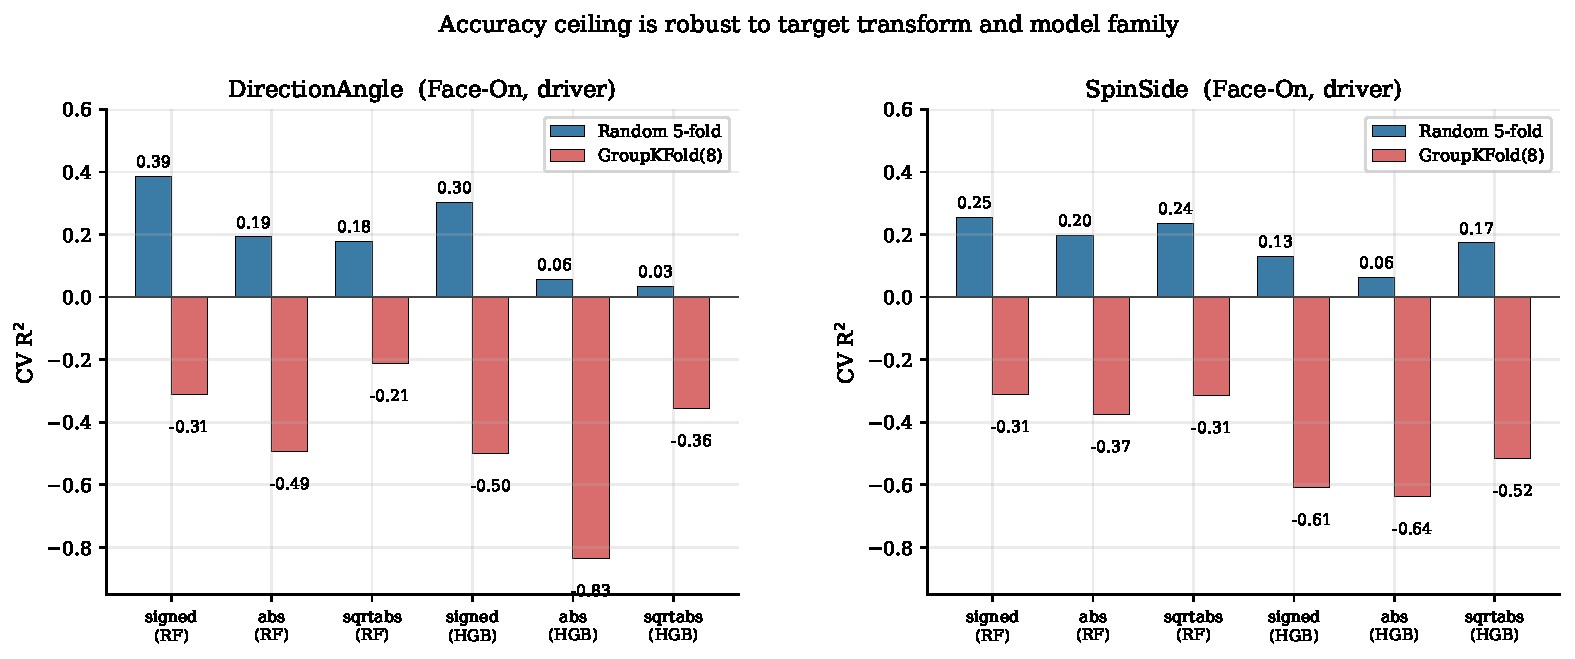
\includegraphics[width=0.98\linewidth]{figures/fig7_robustness.pdf}
\caption{Robustness of the power/accuracy and identity gaps: CV $R^2$ under three target transforms
         (signed, $|y|$, $\sqrt{|y|}$) and two models (Random Forest, HistGradientBoosting), Face-On view.
         Blue = random 5-fold; red = GroupKFold(8).  The identity gap appears in every cell.}
\label{fig:robustness}
\end{figure}

\subsection{Four clusters --- but two are golfer-dominated}
\label{sec:archetypes}

Figure~\ref{fig:archetypes}c reports silhouette vs.\ $K$ with a permuted-label null baseline: the silhouette
is high ($>0.5$) at $K=2\text{--}7$ and uniformly far above null, then drops sharply from $K=7$ to $K=8$,
which matches the number of golfers.  Davies--Bouldin has no clear minimum in the same range.  We fix $K=4$
as a compromise between coarser and finer solutions, but the sweep already hints that much of the clustering
signal lines up with golfer identity.

Figure~\ref{fig:archetypes}a is the UMAP embedding coloured by the four-cluster $K$-means solution.  The
four clusters have silhouette $0.54$ and the following cluster sizes: A0 ($n=33$, mean drive $\approx 156$ yd),
A1 ($n=512$, $\approx 191$ yd), A2 ($n=32$, $\approx 183$ yd), A3 ($n=36$, $\approx 167$ yd).

The per-golfer crosstab (Fig.~\ref{fig:archetypes}b) is where the subject-effect risk becomes explicit:
A3 is 89\% Golfer 4 (32/36), A0 is 82\% Golfer 8 (27/33), A2 is 56\% Golfer 5 (18/32), and A1 is the only
cross-golfer cluster of substantive size (spanning 8/8 golfers with entropy $2.54$ bits out of a maximum of
$\log_2 8 = 3.0$).  Entropy over golfers per cluster: A0 $=0.87$, A1 $=2.54$, A2 $=1.42$, A3 $=0.50$ bits.

Leave-one-golfer-out stability reinforces this: mean Adjusted Rand Index between the full-sample clustering
and an 8-way LOGO refit is $0.956$, but drops to $0.83$ and $0.82$ when Golfer 4 or Golfer 8 is held out ---
the two golfers that dominate A3 and A0.  We therefore refer to the clusters as A0--A3 throughout rather than
as biomechanical archetype names; a population-level ``aggressive rotator'' archetype cannot be claimed from a
cluster that is effectively one golfer.

\begin{figure}[t]
\centering
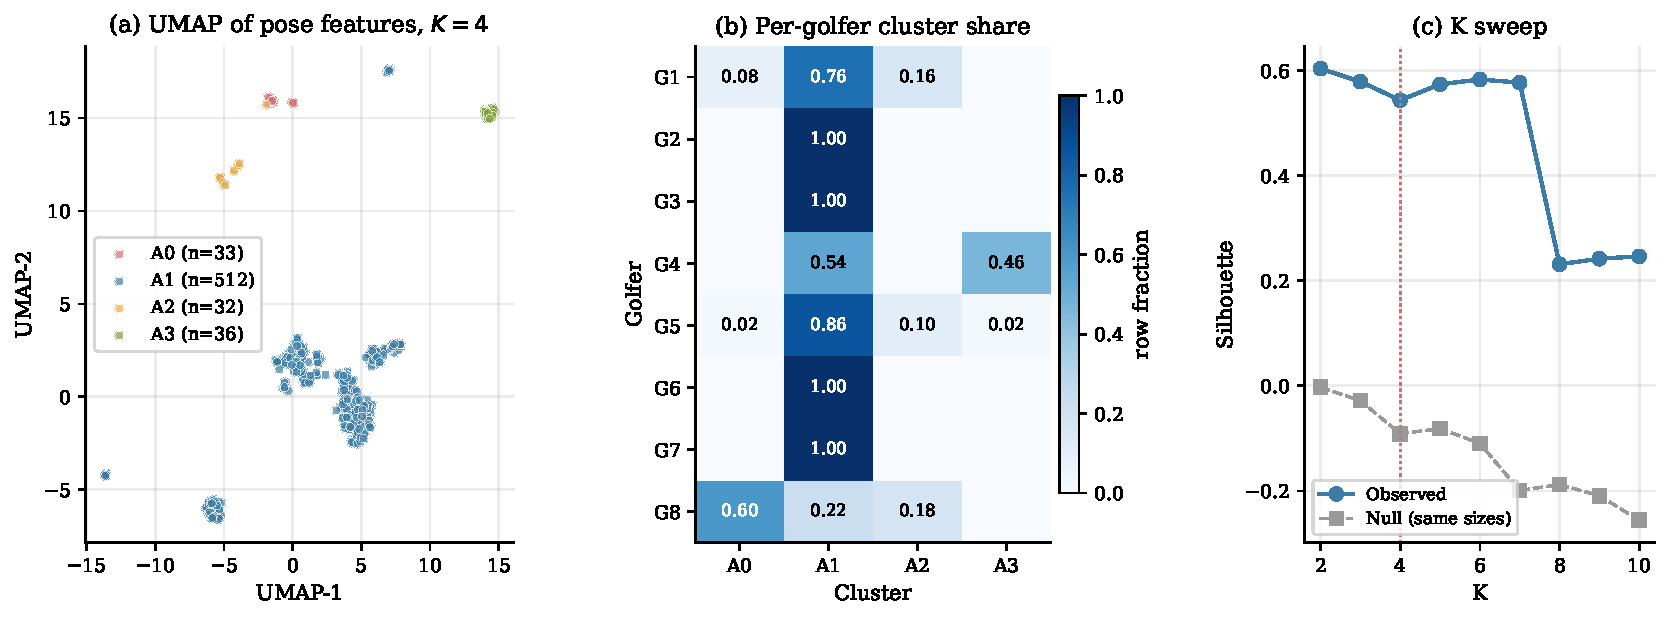
\includegraphics[width=0.99\linewidth]{figures/fig3_archetypes.pdf}
\caption{Cluster validation.  (a) UMAP of the Face-On pose features, coloured by $K=4$ $K$-means.
         (b) Per-golfer $\times$ per-cluster row-fraction heatmap: A0 is $\sim$82\% Golfer 8,
         A3 is $\sim$89\% Golfer 4; A1 is the only cross-golfer cluster.
         (c) Silhouette vs.\ $K$ with a permuted-label null baseline; the observed silhouette is
         well above null at every $K$ but the large drop between $K=7$ and $K=8$ tracks the number of golfers.}
\label{fig:archetypes}
\end{figure}

\subsection{A within-sample rule tree, reported honestly}
\label{sec:rules}

Figure~\ref{fig:tree} shows a depth-3 regression tree ($\texttt{min\_samples\_leaf}=30$) targeting Distance
on the Face-On $\times$ W1 subset.  The tree's cross-validation numbers are telling:
\textbf{random 5-fold CV $R^2=0.34$, GroupKFold(8) CV $R^2=-3.36$}, and the depth sweep (Table~\ref{tab:depth})
shows the pattern is depth-insensitive.  Read in GroupKFold terms, the tree does not generalise across
golfers.  Read in within-sample terms, it compresses the strongest within-corpus associations into a
human-readable structure: \texttt{2-LEFT-ARM-ANGLE}, \texttt{1-HIP-SHIFTED}, and \texttt{4-HIP-SHIFTED}
together define seven leaves whose mean drive distances range from $144.6$ to $227.3$ yards.

\begin{table}[t]
\centering
\small
\caption{Depth sensitivity of the regression-tree surrogate.  Random-CV $R^2$ is roughly flat in depth;
         GroupKFold $R^2$ is uniformly negative and \emph{worsens} at deeper settings, indicating that the
         added leaves chase golfer-specific structure.}
\label{tab:depth}
\begin{tabular}{crr}
\toprule
\textbf{Depth} & \textbf{Random 5-fold $R^2$} & \textbf{GroupKFold(8) $R^2$} \\
\midrule
2 & 0.299 & $-3.47$ \\
3 & 0.338 & $-3.36$ \\
4 & 0.317 & $-3.54$ \\
5 & 0.315 & $-3.61$ \\
\bottomrule
\end{tabular}
\end{table}

Figure~\ref{fig:leaves} plots each leaf's mean Distance with a 95\% bootstrap CI computed from 2{,}000 resamples.
The widest leaves are the small-$n$ leaves at either extreme: the best leaf ($n=37$, mean $227.3$ yd) has a
bootstrap 95\% CI of $[223.0, 231.7]$ yd; the worst ($n=31$, mean $144.6$ yd) has $[139.7, 150.1]$ yd.  The
point-estimate range is therefore real within-sample but narrower than the na\"ive $145 \to 227$ gap
suggests.  A reader-friendly description of the best-leaf rule path:

\begin{tcolorbox}[colback=blue!3,colframe=blue!50!black,
    title={Within-sample rule path to the best leaf (driver, Face-On; NOT a population prescription)}]
\small
\texttt{IF 2-LEFT-ARM-ANGLE > 160.9} \quad\textit{(lead arm within $\sim$19$^{\circ}$ of straight at mid-BS)} \\
\quad\texttt{AND 1-HIP-SHIFTED > -0.52} \quad\textit{(hips not far behind the ball at takeaway)} \\
\quad\texttt{AND 4-HIP-SHIFTED > -0.15} \quad\textit{(hips have begun shifting toward target in early downswing)} \\
$\Rightarrow$ \textbf{predicted leaf mean $\approx 227$ yd} (95\% bootstrap CI $[223, 232]$, $n=37$). \\[2pt]
The worst leaf ($\approx 145$ yd, CI $[140, 150]$, $n=31$) takes the opposite branches at each of these splits.
\end{tcolorbox}

Because GroupKFold $R^2$ is negative, these rules should not be read as
\emph{``if the next golfer sets their hips this way, they will hit it $+82$ yd longer.''}  They should be read
as \emph{``across these 8 golfers, leaves satisfying this conjunction produced long drives; the surrogate
compresses that observation.''}  Section~\ref{sec:limits} returns to this distinction.

\begin{figure}[t]
\centering
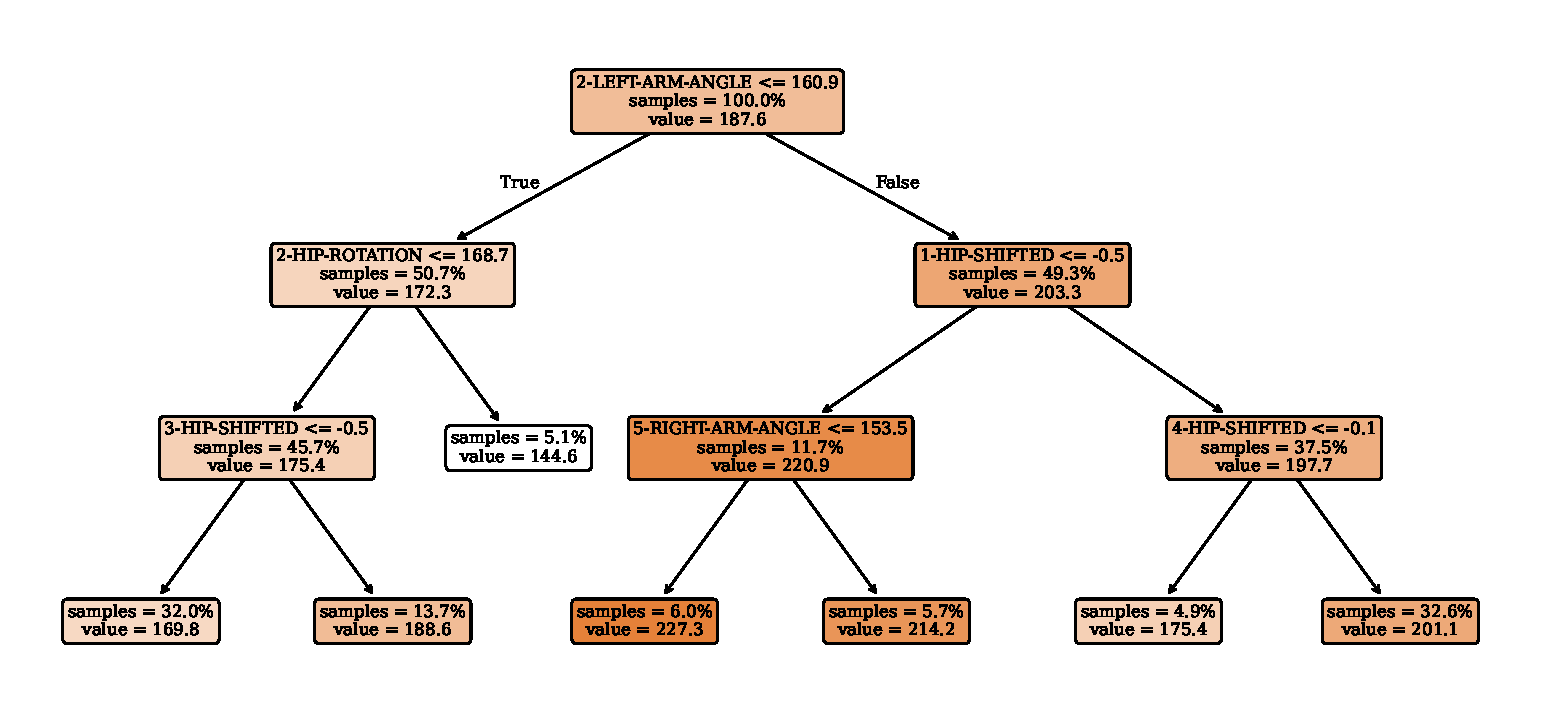
\includegraphics[width=0.88\linewidth]{figures/fig4_tree.pdf}
\caption{Depth-3 regression tree for driver distance, Face-On view.  Leaf labels are the predicted mean distance
         (yards); \texttt{proportion} reports the share of training examples reaching each leaf.  Random CV
         $R^2 = 0.34$; GroupKFold(8) CV $R^2 = -3.36$.}
\label{fig:tree}
\end{figure}

\begin{figure}[t]
\centering
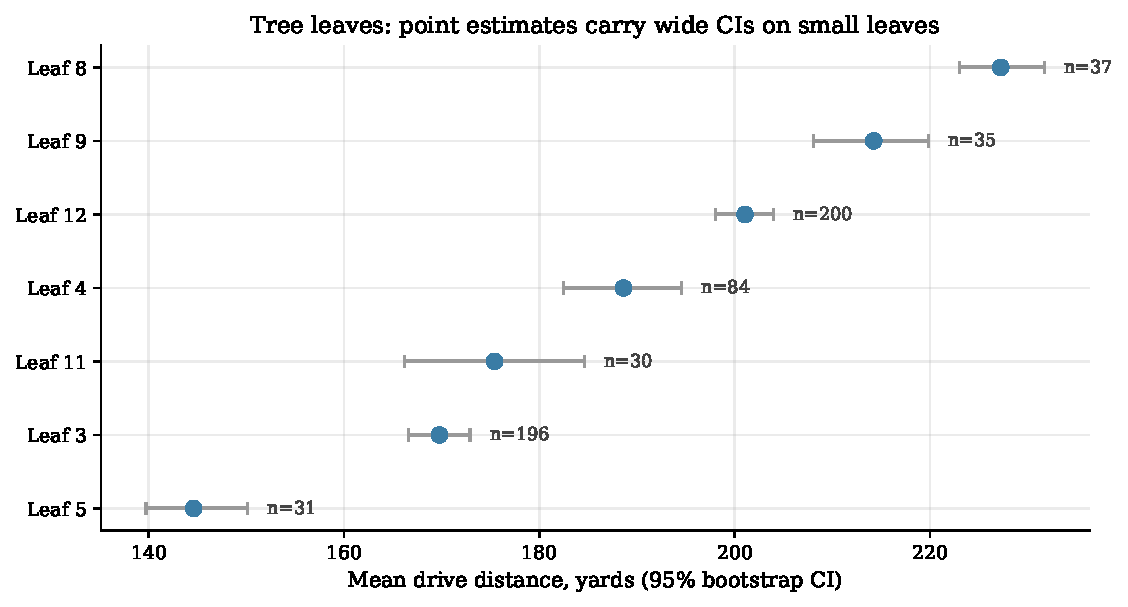
\includegraphics[width=0.78\linewidth]{figures/fig8_tree_leaves.pdf}
\caption{Per-leaf mean Distance and 95\% bootstrap percentile CI.  Sample sizes are annotated at right.
         Small leaves carry wide CIs --- the $145\to 227$ yd spread is real within-sample but is still
         driven by leaves of modest $n$.}
\label{fig:leaves}
\end{figure}

Figure~\ref{fig:distributions} shows, for the six most-discriminating rule features, the top-20\%/bot-20\%
distance histograms overlaid with group medians.  The distributions separate cleanly in modes as well as means,
consistent with the large extreme-groups $d$ reported in the effect-size map --- but with the caveat that the
$d$ statistics shown on each panel overstate the underlying continuous effect.

\begin{figure}[t]
\centering
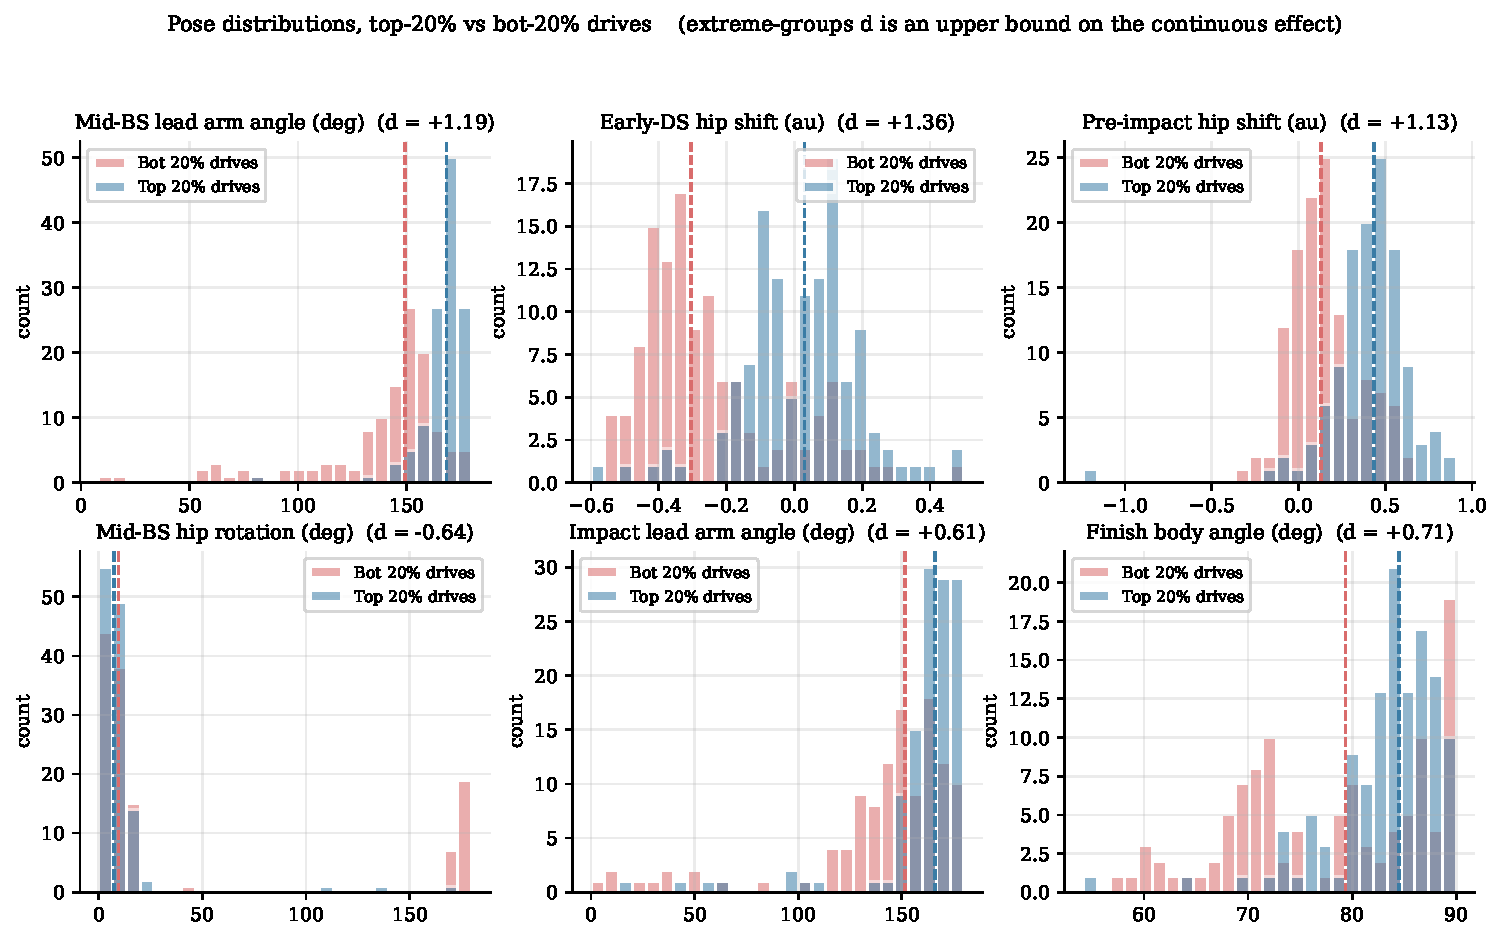
\includegraphics[width=0.99\linewidth]{figures/fig6_distributions.pdf}
\caption{Distributional shifts between long (top 20\%) and short (bottom 20\%) drives across the six
         most-discriminating pose features.  Dashed lines = group medians; $d$ = extreme-groups Cohen's $d$
         (an upper bound on the continuous standardised effect size).}
\label{fig:distributions}
\end{figure}

\section{Discussion}

\paragraph{The identity gap is the main finding.}
The most important number in this paper is not $R^2=0.50$ but the \emph{gap} to $-4.36$.  A predictor that
looks like it recovers half the variance in driver distance on random CV recovers none of it across
unseen golfers.  For the CaddieSet corpus at its current scale, this means pose-only models are
within-subject descriptors, not cross-subject predictors.

\paragraph{What the effect-size map does and does not claim.}
The FDR-surviving associations are real in the sense that they will not be overturned by any reasonable
correction for multiple testing on this grid.  They are also \emph{within-sample} associations: 8 golfers
contribute all variance that the tests see.  Replication on a larger golfer cohort is required before claiming
that a straighter mid-backswing lead arm or an earlier hip shift causes distance at the population level.

\paragraph{Archetypes as mixed style + identity factors.}
The four-cluster solution has internal structure that is well above the null-label baseline and is stable
under LOGO for 6/8 held-out golfers.  But two of the four clusters are effectively single-golfer pools, and
the most biomechanically interesting narrative labels from the first draft of this paper (``Aggressive
Rotator'', ``Early Hip Release'') described patterns that are, in this corpus, barely separable from
``Golfer 5's swing'' and ``Golfer 8's swing'' respectively.  We report the clusters as A0--A3 only, and treat
them as a descriptive partition to be revalidated on a broader corpus.

\paragraph{Rule surrogate as a compression, not a prescription.}
The tree's leaf structure compresses the within-corpus associations into a form that a coach can read, which
has pedagogical value.  But a prescriptive claim --- ``if you do X, your distance will go up Y yards'' ---
cannot be made from data in which the predictor does not cross golfer boundaries.  Our
\href{https://github.com/edwardxiong2027/caddieset-rules}{code release} includes every CV split so the
honest numbers are auditable.

\section{Limitations and Threats to Validity}
\label{sec:limits}

\begin{itemize}
    \item \textbf{Very small golfer pool ($N=8$).}  This is the binding constraint on every inference in the
          paper.  It is why the ceiling analysis collapses under GroupKFold, why two of four clusters are
          single-golfer, and why we avoid the word ``prescription'' throughout the results.
    \item \textbf{Observational data; no intervention.}  All associations are correlational.  A straighter
          lead arm at mid-backswing \emph{could} be a cause of distance, or merely a marker of a golfer whose
          coil already supports distance.  Interventional or repeated-measures studies are required for
          causal coaching claims.
    \item \textbf{Inferred feature semantics.}  The data release does not publish units and sign conventions
          for the pose-feature names; our interpretations follow the most natural biomechanical reading.  If
          a column's sign convention differs from what we assume, the directional narrative (``hips shift
          target-ward'', etc.) would flip, but the effect-size magnitudes would not.
    \item \textbf{Extreme-groups Cohen's $d$ is inflated.}  We report $d$ for continuity with the coaching
          literature, but we also report continuous Pearson $r$, the Fitzsimons back-transform, and Spearman
          $\rho$; the continuous effects are roughly $30\text{--}40\%$ of the $d$ magnitudes.
    \item \textbf{No club-face or path data.}  The accuracy ceiling is capped by features the dataset does not
          include; a secondary high-speed camera at impact would likely lift the accuracy $R^2$.
    \item \textbf{Single-view deployment loses signal.}  Face-On and DTL emphasise different phases; either
          view alone leaves measurable signal on the table.
\end{itemize}

\section{Reproducibility}

Code, artefacts and this manuscript source are released under an MIT licence at
\url{https://github.com/edwardxiong2027/caddieset-rules}.  Seeds are fixed (42); a single \texttt{make}
invocation reproduces every artefact in \texttt{artifacts/} and every figure under \texttt{paper/figures/}.
The underlying CaddieSet data remain the property of \citet{jung2025caddieset} and are used here under their
terms.

\section{Conclusion}

We revisit the CaddieSet corpus with a small-$N$, secondary-analysis lens.  After BH-FDR correction and with
continuous-$r$ back-transforms, mid-backswing lead-arm angle and early/pre-impact hip shift remain the strongest
pose correlates of driver distance, but the largest continuous $r$ is $\approx 0.46$, not $\approx 0.7$.  Under
golfer-aware GroupKFold, every pose-only predictive ceiling on this corpus collapses to negative $R^2$,
indicating that the often-quoted $R^2\approx 0.5$ distance ceiling is identity-dominated at $N=8$.  Clustering
recovers four well-separated partitions, but two of them are effectively one-golfer pools.  A shallow tree
surrogate offers a readable within-sample description, not a population prescription.  CaddieSet is a valuable
resource; its current scale supports descriptive biomechanical claims and motivates collection of a larger,
cross-subject corpus before prescriptive coaching rules are attempted.

\section*{Acknowledgements}
We thank the authors of \citet{jung2025caddieset} for releasing the CaddieSet corpus, and the developers of
\texttt{scikit-learn}, \texttt{umap-learn}, and \texttt{matplotlib} for the open-source tooling that makes this
kind of secondary analysis practical.

\bibliographystyle{plainnat}
\bibliography{references}

\appendix
\section{Top feature tables}
\label{app:tables}

Tables~\ref{tab:top-faceon} and~\ref{tab:top-dtl} report the top-12 pose features by extreme-groups
$|d|$ between top-20\% and bottom-20\% driver-distance groups, together with the Fitzsimons continuous-$r$
back-transform and the BH-FDR $q$-value (Pearson).

\begin{table}[h]
\centering
\small
\caption{Top-12 Face-On pose features ranked by $|d|$ ($n_\text{top}=n_\text{bot}=123$).
         $r_{\text{cont}}$ is the Fitzsimons continuous-$r$ back-transform; $q_{\text{FDR}}$ is the BH-FDR
         $q$-value computed on the 252-cell grid.  All rows shown have $q_{\text{FDR}}<0.01$.}
\label{tab:top-faceon}
\begin{tabular}{lrrrrrr}
\toprule
\textbf{Feature} & \textbf{Top mean} & \textbf{Bot mean} & $\boldsymbol{d}$ & $\boldsymbol{r_{\text{pb}}}$ & $\boldsymbol{r_{\text{cont}}}$ & $\boldsymbol{q_{\text{FDR}}}$ \\
\midrule
4-HIP-SHIFTED        & $+0.018$        & $-0.245$        & $+1.36$ & $+0.56$ & $+0.45$ & ${<}10^{-4}$ \\
2-LEFT-ARM-ANGLE     & $167.9^{\circ}$ & $139.2^{\circ}$ & $+1.19$ & $+0.50$ & $+0.39$ & ${<}10^{-4}$ \\
5-HIP-SHIFTED        & $+0.407$        & $+0.155$        & $+1.13$ & $+0.49$ & $+0.37$ & ${<}10^{-4}$ \\
7-FINISH-ANGLE       & $83.3^{\circ}$  & $78.0^{\circ}$  & $+0.71$ & $+0.33$ & $+0.22$ & ${<}10^{-3}$ \\
6-RIGHT-LEG-ANGLE    & $159.0^{\circ}$ & $164.4^{\circ}$ & $-0.67$ & $-0.31$ & $-0.20$ & ${<}10^{-3}$ \\
1-LEFT-ARM-ANGLE     & $169.1^{\circ}$ & $158.5^{\circ}$ & $+0.64$ & $+0.30$ & $+0.19$ & ${<}10^{-3}$ \\
2-HIP-ROTATION       & $10.6^{\circ}$  & $43.3^{\circ}$  & $-0.64$ & $-0.30$ & $-0.19$ & ${<}10^{-3}$ \\
3-HIP-SHIFTED        & $-0.447$        & $-0.599$        & $+0.64$ & $+0.30$ & $+0.19$ & ${<}10^{-3}$ \\
2-SHOULDER-LOC       & $58.1$          & $34.9$          & $+0.63$ & $+0.30$ & $+0.19$ & ${<}10^{-3}$ \\
3-RIGHT-LEG-ANGLE    & $167.3^{\circ}$ & $173.7^{\circ}$ & $-0.61$ & $-0.29$ & $-0.18$ & ${<}10^{-3}$ \\
6-LEFT-ARM-ANGLE     & $161.1^{\circ}$ & $140.8^{\circ}$ & $+0.61$ & $+0.29$ & $+0.18$ & ${<}10^{-3}$ \\
6-HIP-SHIFTED        & $+0.459$        & $+0.254$        & $+0.54$ & $+0.26$ & $+0.16$ & ${<}10^{-2}$ \\
\bottomrule
\end{tabular}
\end{table}

\begin{table}[h]
\centering
\small
\caption{Top-12 Down-the-Line pose features ($n_\text{top}=108$, $n_\text{bot}=105$).  Columns as in
         Table~\ref{tab:top-faceon}.}
\label{tab:top-dtl}
\begin{tabular}{lrrrrrr}
\toprule
\textbf{Feature} & \textbf{Top mean} & \textbf{Bot mean} & $\boldsymbol{d}$ & $\boldsymbol{r_{\text{pb}}}$ & $\boldsymbol{r_{\text{cont}}}$ & $\boldsymbol{q_{\text{FDR}}}$ \\
\midrule
3-RIGHT-DISTANCE    & $0.670$         & $0.582$         & $+1.54$ & $+0.61$ & $+0.50$ & ${<}10^{-4}$ \\
3-RIGHT-LEG-ANGLE   & $167.2^{\circ}$ & $177.6^{\circ}$ & $-1.40$ & $-0.57$ & $-0.46$ & ${<}10^{-4}$ \\
0-SPINE-ANGLE       & $73.2^{\circ}$  & $77.9^{\circ}$  & $-1.11$ & $-0.48$ & $-0.36$ & ${<}10^{-4}$ \\
3-RIGHT-ARM-ANGLE   & $75.8^{\circ}$  & $64.1^{\circ}$  & $+0.90$ & $+0.41$ & $+0.29$ & ${<}10^{-4}$ \\
1-SPINE-ANGLE       & $75.8^{\circ}$  & $78.4^{\circ}$  & $-0.81$ & $-0.38$ & $-0.26$ & ${<}10^{-3}$ \\
4-HIP-ANGLE         & $6.5^{\circ}$   & $11.2^{\circ}$  & $-0.76$ & $-0.35$ & $-0.24$ & ${<}10^{-3}$ \\
5-LEFT-LEG-ANGLE    & $175.1^{\circ}$ & $169.6^{\circ}$ & $+0.74$ & $+0.35$ & $+0.24$ & ${<}10^{-3}$ \\
6-HIP-ANGLE         & $12.5^{\circ}$  & $18.0^{\circ}$  & $-0.73$ & $-0.34$ & $-0.23$ & ${<}10^{-3}$ \\
7-SHOULDER-ANGLE    & $7.3^{\circ}$   & $12.9^{\circ}$  & $-0.69$ & $-0.32$ & $-0.21$ & ${<}10^{-3}$ \\
3-HIP-ANGLE         & $6.9^{\circ}$   & $9.7^{\circ}$   & $-0.63$ & $-0.30$ & $-0.19$ & ${<}10^{-3}$ \\
6-SPINE-ANGLE       & $80.6^{\circ}$  & $77.0^{\circ}$  & $+0.61$ & $+0.29$ & $+0.18$ & ${<}10^{-3}$ \\
2-SHOULDER-ANGLE    & $18.9^{\circ}$  & $21.1^{\circ}$  & $-0.40$ & $-0.20$ & $-0.12$ & ${<}0.05$ \\
\bottomrule
\end{tabular}
\end{table}

\end{document}
